\documentclass[12pt,a4paper]{article}
\usepackage{fontspec}
\setmainfont{TeX Gyre Termes}
\usepackage[a4paper,margin=2.2cm]{geometry}
\usepackage{graphicx}
\usepackage{float}
\usepackage{booktabs}
\usepackage{longtable}
\usepackage{array}
\usepackage{fancyhdr}
\usepackage{hyperref}
\usepackage{amsmath}
\usepackage{enumitem}
\hypersetup{colorlinks=true, linkcolor=blue, urlcolor=blue}
\setlength{\parindent}{0pt}
\setlength{\parskip}{6pt}
\renewcommand{\arraystretch}{1.25}
\setlength{\headheight}{15pt}

\pagestyle{fancy}
\fancyhf{}
\fancyfoot[C]{\thepage}
\renewcommand{\headrulewidth}{0pt}

\begin{document}

\begin{titlepage}
    \thispagestyle{empty}
    \centering

    \vspace*{1.5cm}
    \IfFileExists{../../../../../assets/rsz_logo-khtn.png}
    {
\includegraphics[width=3.2cm]{../../../../../assets/rsz_logo-khtn.png}\par}
    {\vspace{3.2cm}\par}
    \vspace{0.8cm}

    {\Large\bfseries ĐẠI HỌC QUỐC GIA THÀNH PHỐ HỒ CHÍ MINH\par}
    \vspace{0.2cm}
    {\Large\bfseries TRƯỜNG ĐẠI HỌC KHOA HỌC TỰ NHIÊN\par}
    \vspace{0.15cm}
    {\large KHOA CÔNG NGHỆ THÔNG TIN\par}

    \vspace{2.0cm}
    {\Large\bfseries BÁO CÁO THỰC HÀNH 03\par}
    \vspace{0.4cm}
    {\large\bfseries Phát hiện đối tượng trên ảnh bàn cờ bằng YOLO, DETR và Faster R-CNN\par}

    \vspace{1.8cm}
    \begin{tabular}{>{\bfseries}l l}
        Nhóm: & Myopia \\
        MSHV 1: & 25C11067 - Nguyễn Thái Thông \\
        MSHV 2: & 25C11035 - Trần Hạ Khánh Duy
    \end{tabular}

    \vfill
    {\large TP. Hồ Chí Minh, 2026\par}
\end{titlepage}
\clearpage
\pagenumbering{arabic}

\section{Mục tiêu}

Bài thực hành 03 tập trung vào bài toán phát hiện đối tượng (object detection) trên bộ dữ liệu ảnh bàn cờ có các quân cờ ở nhiều trạng thái sắp xếp khác nhau. Nhóm xây dựng một pipeline hoàn chỉnh gồm chuẩn hóa dữ liệu, huấn luyện ba mô hình phát hiện đối tượng, xuất ảnh dự đoán và đánh giá kết quả bằng các biểu đồ trực quan.

Các mục tiêu chính của bài gồm:
\begin{itemize}[leftmargin=1.2cm]
    \item tìm hiểu cấu trúc dữ liệu nhãn cho bài toán detection và chuyển đổi giữa các định dạng annotation khác nhau;
    \item cài đặt, huấn luyện và so sánh ba mô hình YOLO, DETR và Faster R-CNN trên cùng một bộ ảnh;
    \item xuất ảnh prediction, confusion matrix và đường cong đánh giá để phục vụ báo cáo;
    \item quan sát ảnh hưởng của dữ liệu mất cân bằng lớp, số lượng object trên ảnh và đặc điểm từng mô hình đến chất lượng dự đoán.
\end{itemize}

Bộ dữ liệu sử dụng trong thực nghiệm gồm 693 ảnh, chia thành 606 ảnh train, 58 ảnh validation và 29 ảnh test. Tổng số bounding box là 7{,}086. Dữ liệu có 13 lớp quân cờ, trong đó một số lớp xuất hiện rất ít như \texttt{bishop}, làm cho bài toán có tính mất cân bằng rõ rệt.

\section{Phân công đóng góp}

\begin{longtable}{p{0.24\textwidth}p{0.68\textwidth}}
\toprule
\textbf{Thành viên} & \textbf{Nội dung đóng góp} \\
\midrule
Nguyễn Thái Thông & Chuẩn bị notebook, triển khai pipeline tiền xử lý dữ liệu, huấn luyện YOLO và DETR, lưu các hình kết quả, hoàn thiện phần đánh giá. \\
Trần Hạ Khánh Duy & Triển khai Faster R-CNN, kiểm tra định dạng annotation, đối chiếu kết quả dự đoán và hoàn thiện phần nhận xét báo cáo. \\
\bottomrule
\end{longtable}

\section{Bảng tự đánh giá}

\begin{longtable}{p{0.24\textwidth}p{0.18\textwidth}p{0.48\textwidth}}
\toprule
\textbf{Thành viên} & \textbf{Mức đóng góp} & \textbf{Ghi chú} \\
\midrule
Nguyễn Thái Thông & 100\% & Hoàn thành phần được phân công, phối hợp kiểm tra pipeline và hình minh chứng. \\
Trần Hạ Khánh Duy & 100\% & Hoàn thành phần được phân công, phối hợp rà soát kết quả huấn luyện và báo cáo. \\
\bottomrule
\end{longtable}

\section{Cơ sở lý thuyết và cách cài đặt}

\subsection{Tổng quan dữ liệu và tiền xử lý}

Dữ liệu gốc được lưu theo ba split \texttt{train}, \texttt{valid} và \texttt{test}. Mỗi ảnh đi kèm các nhãn bounding box tuyệt đối theo dạng \texttt{x1,y1,x2,y2,class\_id}. Khi huấn luyện, nhóm chuyển dữ liệu sang các định dạng phù hợp với từng mô hình:
\begin{itemize}[leftmargin=1.2cm]
    \item YOLO nhận nhãn theo định dạng chuẩn \texttt{class cx cy w h} và được sinh ra từ file \texttt{data.yaml};
    \item DETR sử dụng \texttt{DetrImageProcessor} để encode ảnh và annotation sang format mà Hugging Face mong đợi;
    \item Faster R-CNN dùng trực tiếp bounding box tuyệt đối và label id tăng từ 1 để chừa lớp nền.
\end{itemize}

Trên notebook, nhóm cũng xây dựng các hàm tiện ích để đọc ảnh, hiển thị ảnh, tạo grid minh họa và thống kê dữ liệu. Các hình thống kê cơ bản của bộ dữ liệu gồm ảnh mẫu, phân bố số lượng ảnh theo split và phân bố lớp quân cờ.

\subsection{YOLO}

YOLO là mô hình một giai đoạn (one-stage detector), dự đoán trực tiếp vị trí và nhãn đối tượng trên ảnh đầu vào. Ưu điểm nổi bật của YOLO là tốc độ huấn luyện và suy luận nhanh, phù hợp với các bài toán cần phản hồi gần thời gian thực.

Trong pipeline của bài thực hành, nhóm dùng \texttt{yolov8n.pt} làm backbone pretrain và fine-tune trên dữ liệu cờ vua. Khi huấn luyện, ảnh được resize về cùng kích thước đầu vào, còn nhãn được chuyển sang định dạng YOLO. Việc suy luận dùng ngưỡng confidence thấp hơn để giữ lại nhiều dự đoán hữu ích hơn khi vẽ báo cáo.

\subsection{DETR}

DETR (Detection Transformer) là mô hình detection dựa trên transformer, xem bài toán phát hiện đối tượng như một bài toán dự đoán tập các object không trùng lặp. Khác với YOLO, DETR không phụ thuộc mạnh vào anchor hay các bước hậu xử lý thủ công như NMS trong pipeline cổ điển.

Trong notebook, nhóm dùng \texttt{DetrForObjectDetection} và \texttt{DetrImageProcessor} của Hugging Face để fine-tune trực tiếp trên tập ảnh bàn cờ. Do DETR khá nhạy với learning rate lớn và mixed precision trên tập dữ liệu nhỏ, quá trình train được cấu hình thận trọng hơn với \texttt{fp16=False}, learning rate thấp và gradient clipping.

\subsection{Faster R-CNN}

Faster R-CNN là mô hình hai giai đoạn (two-stage detector) gồm bước đề xuất vùng quan tâm và bước phân lớp chi tiết. So với DETR, Faster R-CNN thường ổn định hơn trong thực nghiệm nhỏ, đặc biệt khi số lớp không quá nhiều.

Nhóm sử dụng backbone pretrain của TorchVision và thay đầu ra classifier cho đúng số lớp quân cờ. Dữ liệu được đưa vào \texttt{DataLoader} theo kiểu batch detection, trong đó mỗi ảnh có số bounding box khác nhau.

\subsection{Đánh giá và xuất kết quả}

Sau khi huấn luyện, nhóm xuất ra bốn nhóm kết quả:
\begin{itemize}[leftmargin=1.2cm]
    \item biểu đồ train/eval loss hoặc metric curve;
    \item confusion matrix trên tập test;
    \item ảnh prediction mẫu cho 5 ảnh test đã chọn;
    \item các panel so sánh giữa YOLO, DETR và Faster R-CNN trên cùng một bộ ảnh test.
\end{itemize}

Mục tiêu của phần đánh giá không chỉ là nhìn số liệu, mà còn quan sát trực quan xem mô hình nào giữ được nhiều quân cờ hơn, mô hình nào nhầm lớp, và mô hình nào phù hợp hơn với ảnh có ít object hoặc ảnh có quân cờ bị che khuất.

\section{Quy trình thực nghiệm}

Quy trình thực nghiệm của bài được thực hiện theo các bước:
\begin{enumerate}[leftmargin=1.2cm]
    \item đọc file nhãn gốc và thống kê số lượng ảnh, số box, số lớp;
    \item hiển thị một số ảnh mẫu và ảnh ground truth để kiểm tra chất lượng annotation;
    \item huấn luyện YOLO, DETR và Faster R-CNN trên cùng bộ dữ liệu;
    \item dùng cùng một tập test image để xuất prediction của ba mô hình;
    \item lưu confusion matrix, evaluation curve và các ảnh so sánh trực quan;
    \item tổng hợp nhận xét về ưu và nhược điểm của từng mô hình.
\end{enumerate}

Nhóm chọn 5 ảnh test tiêu biểu để so sánh giữa ba mô hình. Các ảnh này được lấy từ cùng một danh sách test image nhằm đảm bảo tính công bằng khi so sánh. Ngoài ra, hai ảnh khó nhất còn được tách riêng để tạo panel lỗi, giúp nhìn rõ hơn trường hợp nào mô hình dự đoán thiếu hoặc dự đoán nhầm lớp.

\section{Kết quả và nhận xét}

\subsection{Tổng quan bộ dữ liệu}

Các ảnh mẫu trong bộ dữ liệu cho thấy quân cờ thường xuất hiện trên nền bàn cờ khá đều màu, nhưng có thể bị che khuất một phần, chồng lấn hoặc xuất hiện với nhiều góc nhìn khác nhau. Đây là lý do khiến bài toán detection trên ảnh bàn cờ không hoàn toàn đơn giản dù số lớp chỉ ở mức trung bình.

\begin{figure}[H]
    \centering
    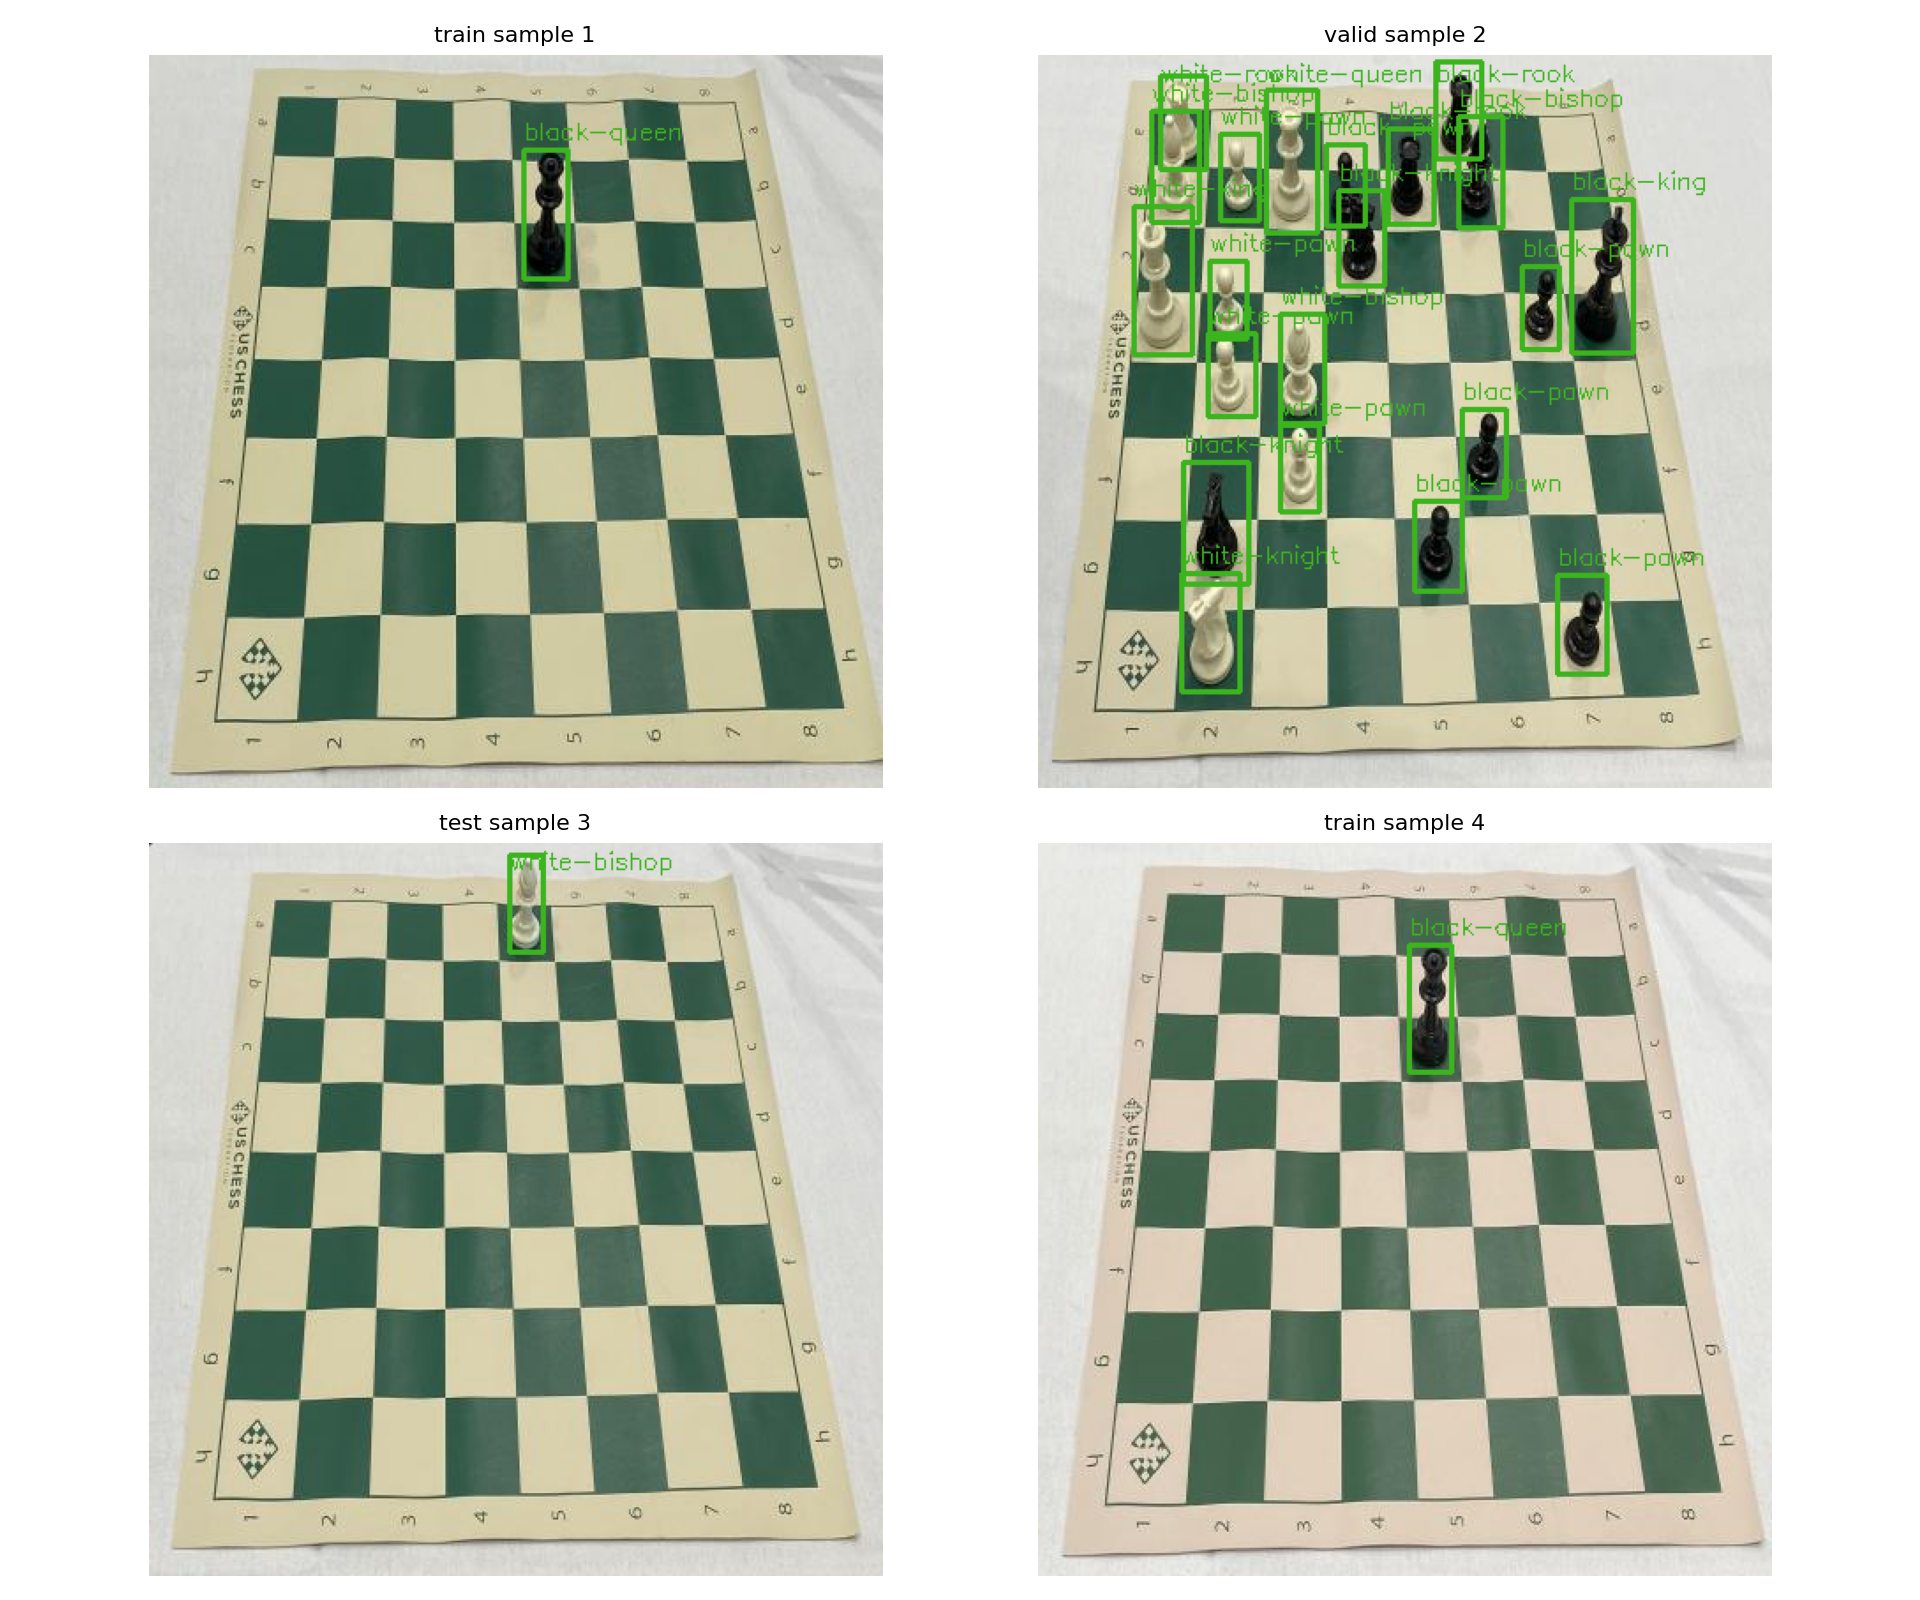
\includegraphics[width=\textwidth]{figures/dataset_samples_grid.png}
    \caption{Một số ảnh mẫu của bộ dữ liệu.}
\end{figure}

\begin{figure}[H]
    \centering
    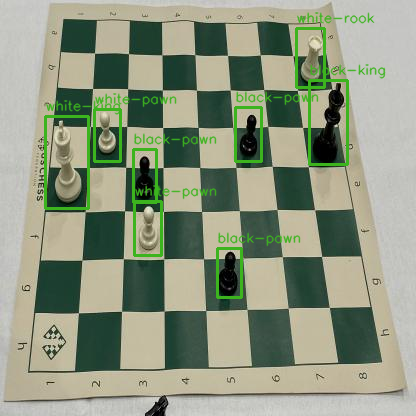
\includegraphics[width=0.86\textwidth]{figures/sample_ground_truth.png}
    \caption{Một ảnh ground truth tiêu biểu sau khi gắn bounding box.}
\end{figure}

\begin{figure}[H]
    \centering
    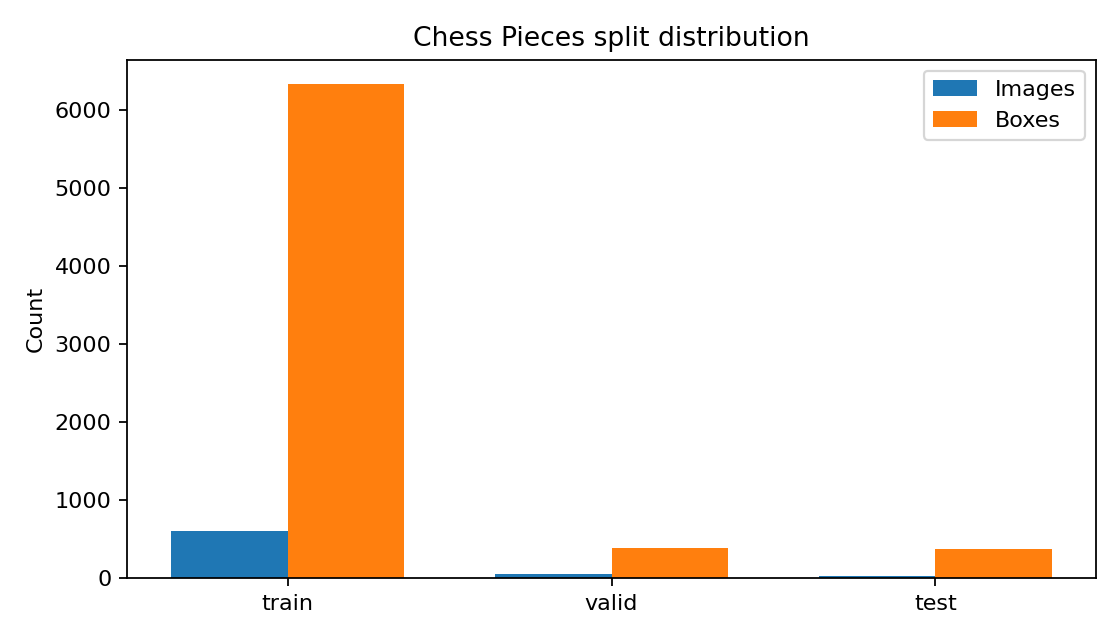
\includegraphics[width=0.78\textwidth]{figures/split_distribution.png}
    \caption{Phân bố số ảnh và số bounding box theo từng split.}
\end{figure}

\begin{figure}[H]
    \centering
    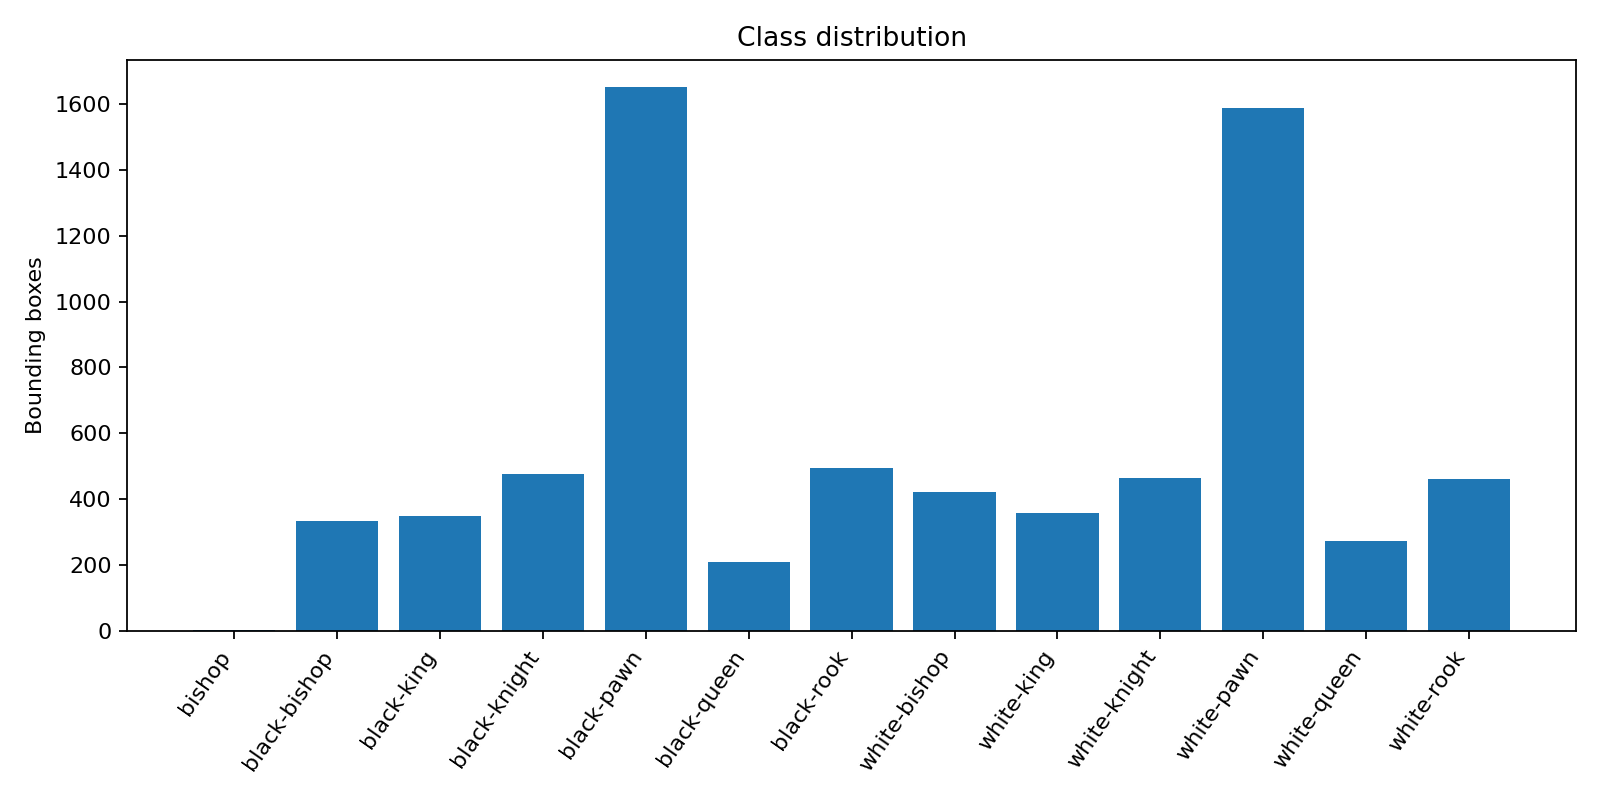
\includegraphics[width=0.86\textwidth]{figures/class_distribution.png}
    \caption{Phân bố số bounding box theo lớp.}
\end{figure}

Từ biểu đồ phân bố lớp, có thể thấy dữ liệu bị lệch mạnh: một số lớp như \texttt{black-pawn} và \texttt{white-pawn} xuất hiện rất nhiều, trong khi \texttt{bishop} gần như không có mẫu. Đây là nguyên nhân quan trọng khiến các mô hình học khó đồng đều trên toàn bộ lớp, đặc biệt với lớp hiếm.

\subsection{So sánh trực quan giữa ba mô hình}

Toàn bộ đánh giá định lượng trong bài đều được tính trên cùng tập \texttt{test}. Confusion matrix, đường cong đánh giá và các ảnh prediction đều dùng chung bộ test image, cùng ngưỡng confidence trong quá trình hiển thị, nên có thể so sánh trực tiếp giữa ba mô hình.

\subsubsection{Confusion matrix}

Ở bảng confusion matrix, YOLO giữ được xu hướng đường chéo khá rõ và ít ô nền hơn hai mô hình còn lại. DETR có xu hướng thận trọng hơn, dẫn đến một số lớp bị bỏ sót và xuất hiện nhiều dự đoán đi vào cột nền. Faster R-CNN có độ phủ tốt, nhưng trong một vài lớp gần nhau vẫn có nhầm lẫn nhẹ.

\begin{figure}[H]
    \centering
    \begin{minipage}[t]{0.32\textwidth}
        \centering
        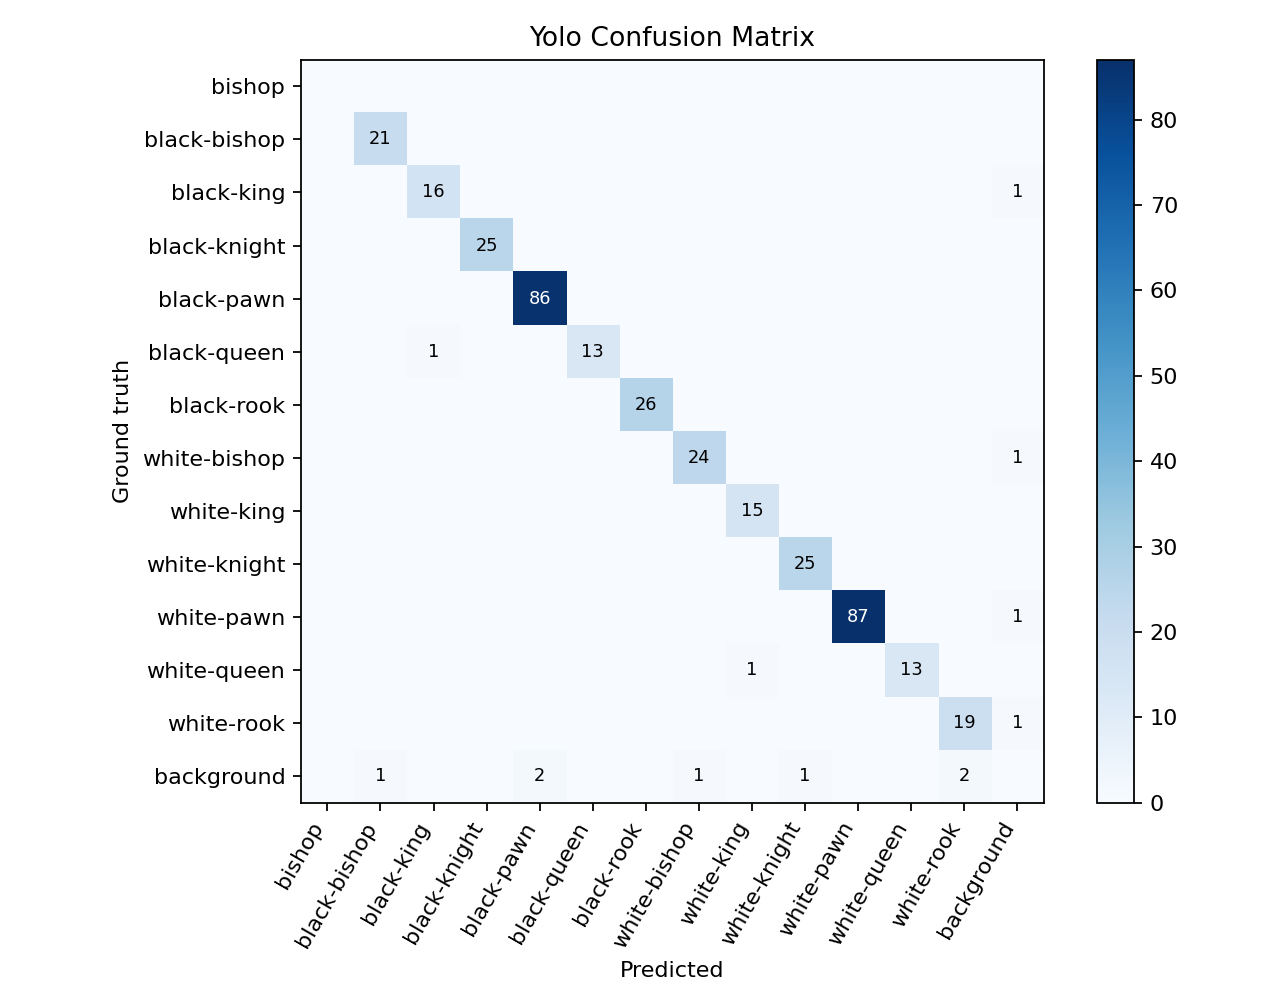
\includegraphics[width=\textwidth]{figures/yolo_confusion_matrix.png}
        \small YOLO
    \end{minipage}\hfill
    \begin{minipage}[t]{0.32\textwidth}
        \centering
        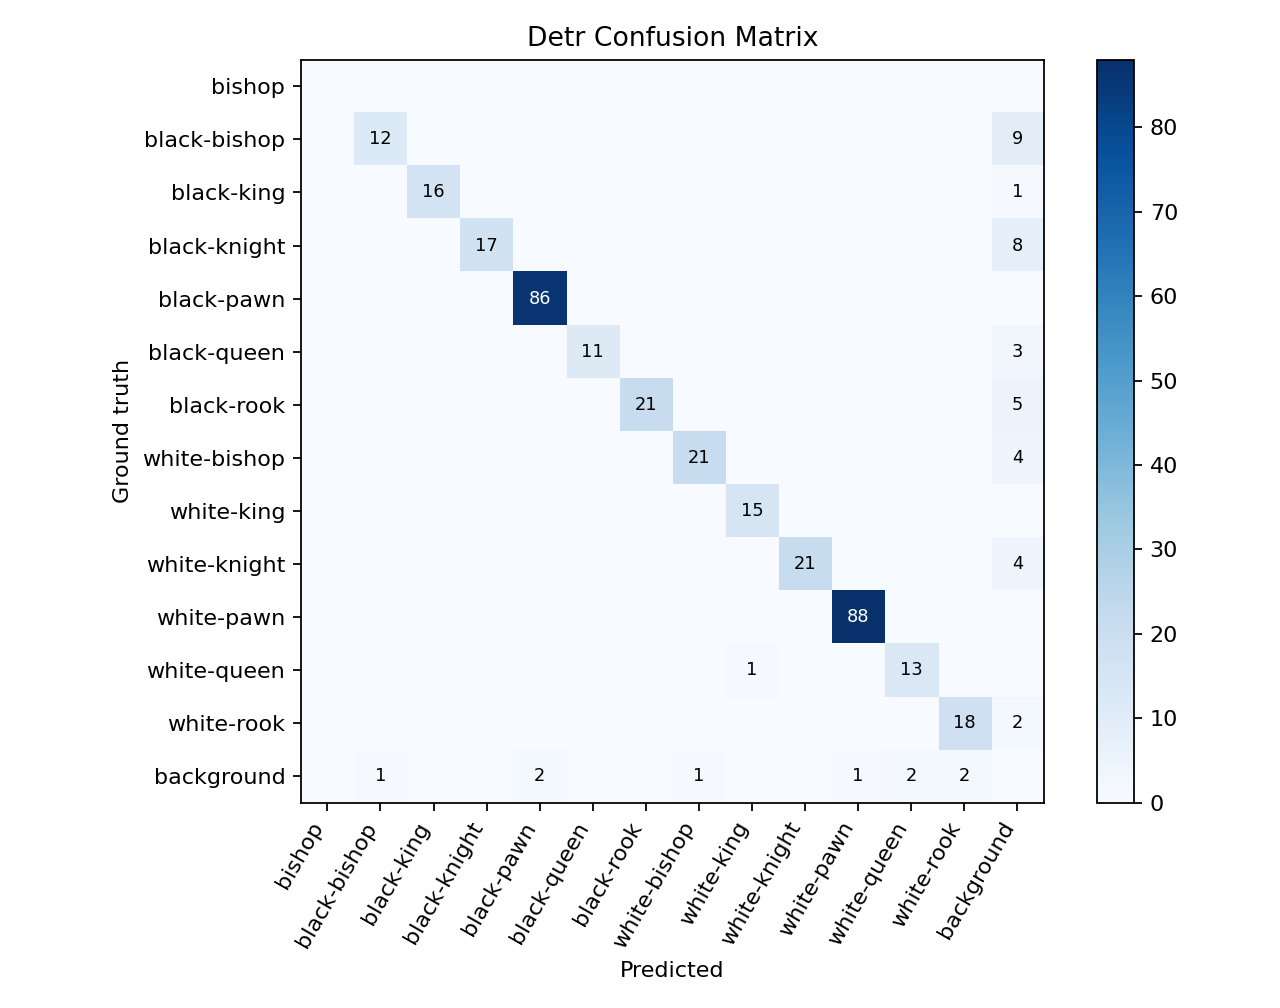
\includegraphics[width=\textwidth]{figures/detr_confusion_matrix.png}
        \small DETR
    \end{minipage}\hfill
    \begin{minipage}[t]{0.32\textwidth}
        \centering
        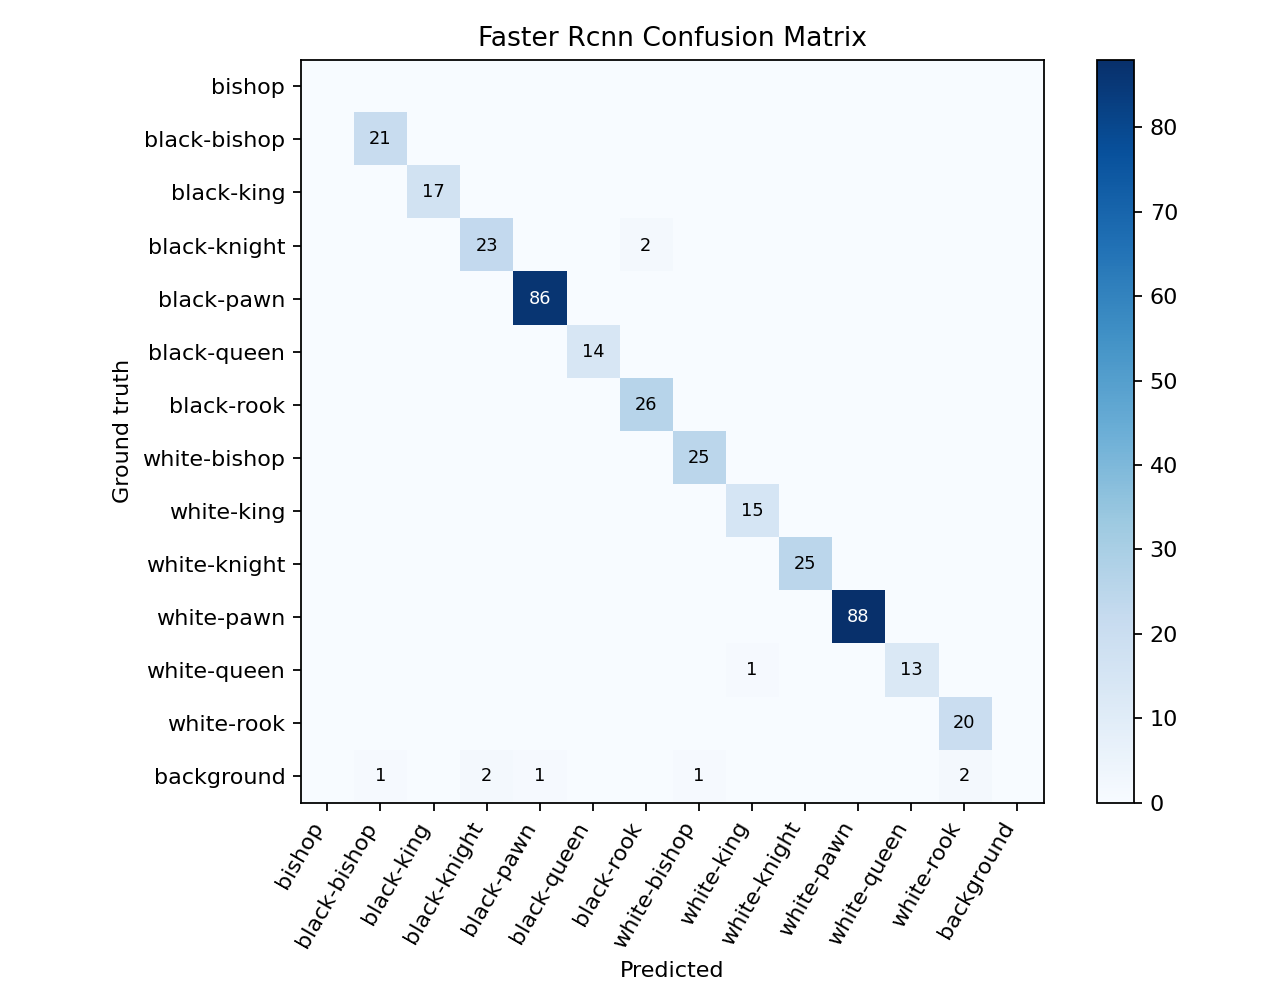
\includegraphics[width=\textwidth]{figures/faster_rcnn_confusion_matrix.png}
        \small Faster R-CNN
    \end{minipage}
    \caption{So sánh confusion matrix của ba mô hình trên cùng tập test.}
\end{figure}

Trong ba mô hình, YOLO và Faster R-CNN cho số lượng dự đoán đúng khá ổn định ở các lớp phổ biến như \texttt{black-pawn} và \texttt{white-pawn}. DETR vẫn nhận ra được cấu trúc chung nhưng thiên về dự đoán ít box hơn, đặc biệt ở các ảnh ít object hoặc object nhỏ.

\subsubsection{Prediction theo cùng ảnh test}

Nhóm dùng cùng 5 ảnh test tiêu biểu để nhìn prediction của cả ba mô hình theo từng case. Cách trình bày này giúp nhận ra rất rõ sự khác nhau giữa các model trong cùng điều kiện đầu vào.

Case 1 là ảnh gần như trống, nên cả ba mô hình đều không tạo ra prediction đáng kể. Đây là case hợp lý để kiểm tra xu hướng false positive của model.

\begin{figure}[H]
    \centering
    \begin{minipage}[t]{0.32\textwidth}
        \centering
        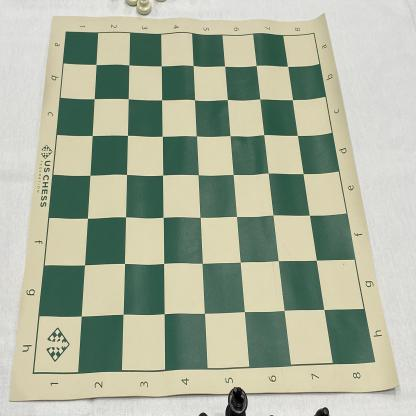
\includegraphics[width=\textwidth]{figures/yolo_prediction_1.png}
        \small YOLO
    \end{minipage}\hfill
    \begin{minipage}[t]{0.32\textwidth}
        \centering
        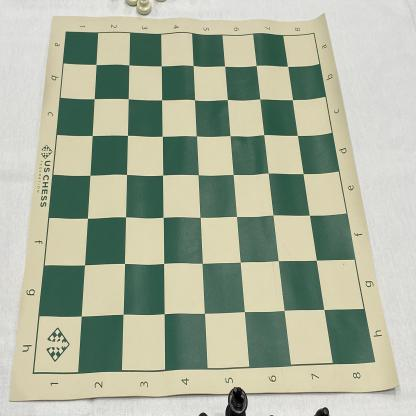
\includegraphics[width=\textwidth]{figures/detr_prediction_1.png}
        \small DETR
    \end{minipage}\hfill
    \begin{minipage}[t]{0.32\textwidth}
        \centering
        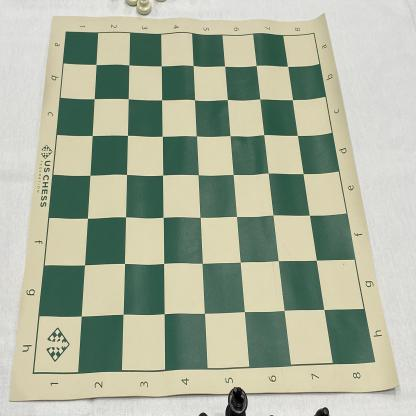
\includegraphics[width=\textwidth]{figures/faster_rcnn_prediction_1.png}
        \small Faster R-CNN
    \end{minipage}
    \caption{So sánh prediction trên test case 1.}
\end{figure}

Case 2 có một quân đen ở giữa bàn cờ. Cả ba mô hình đều bắt được object chính, trong đó YOLO và Faster R-CNN cho bounding box gọn và rõ, còn DETR cũng đúng nhưng thường ít box phụ hơn.

\begin{figure}[H]
    \centering
    \begin{minipage}[t]{0.32\textwidth}
        \centering
        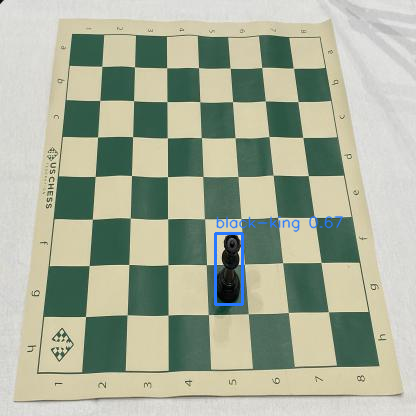
\includegraphics[width=\textwidth]{figures/yolo_prediction_2.png}
        \small YOLO
    \end{minipage}\hfill
    \begin{minipage}[t]{0.32\textwidth}
        \centering
        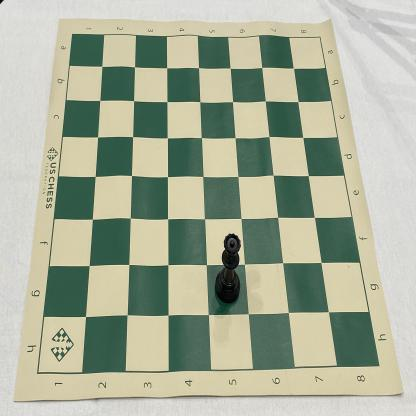
\includegraphics[width=\textwidth]{figures/detr_prediction_2.png}
        \small DETR
    \end{minipage}\hfill
    \begin{minipage}[t]{0.32\textwidth}
        \centering
        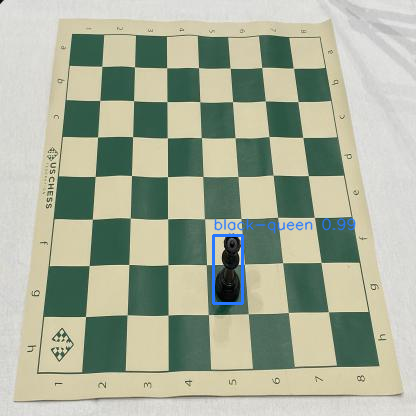
\includegraphics[width=\textwidth]{figures/faster_rcnn_prediction_2.png}
        \small Faster R-CNN
    \end{minipage}
    \caption{So sánh prediction trên test case 2.}
\end{figure}

Case 3 có một quân trắng sát mép trên. YOLO và Faster R-CNN vẫn giữ được prediction đúng, còn DETR dự đoán được nhưng thường gọn hơn, thể hiện đúng tính thận trọng của mô hình.

\begin{figure}[H]
    \centering
    \begin{minipage}[t]{0.32\textwidth}
        \centering
        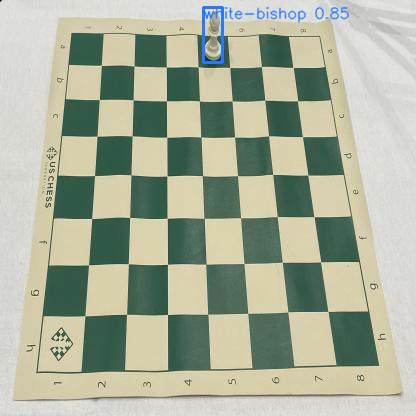
\includegraphics[width=\textwidth]{figures/yolo_prediction_3.png}
        \small YOLO
    \end{minipage}\hfill
    \begin{minipage}[t]{0.32\textwidth}
        \centering
        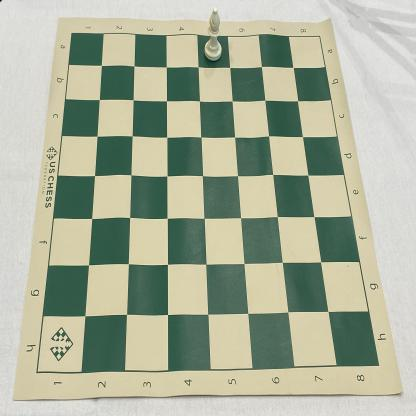
\includegraphics[width=\textwidth]{figures/detr_prediction_3.png}
        \small DETR
    \end{minipage}\hfill
    \begin{minipage}[t]{0.32\textwidth}
        \centering
        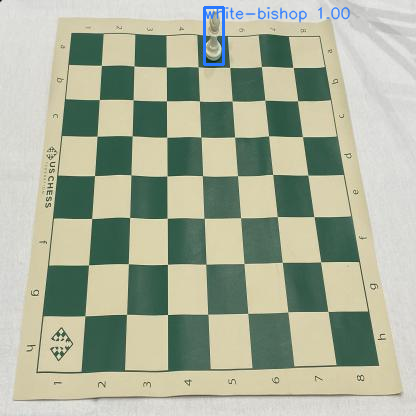
\includegraphics[width=\textwidth]{figures/faster_rcnn_prediction_3.png}
        \small Faster R-CNN
    \end{minipage}
    \caption{So sánh prediction trên test case 3.}
\end{figure}

Case 4 là ảnh khó hơn, có nhiều quân cùng xuất hiện. Ở case này, YOLO vẫn giữ được khá nhiều detection, DETR có xu hướng rơi vào tình trạng dự đoán dày nhưng không đều bằng YOLO, còn Faster R-CNN khá mạnh ở việc giữ box của các quân chính.

\begin{figure}[H]
    \centering
    \begin{minipage}[t]{0.32\textwidth}
        \centering
        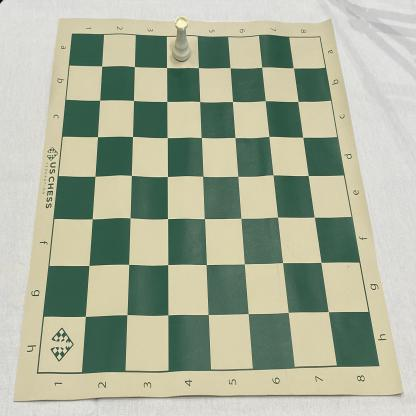
\includegraphics[width=\textwidth]{figures/yolo_prediction_4.png}
        \small YOLO
    \end{minipage}\hfill
    \begin{minipage}[t]{0.32\textwidth}
        \centering
        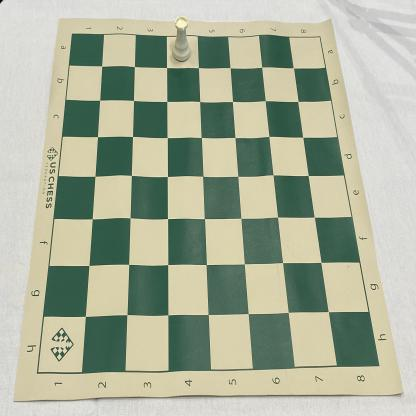
\includegraphics[width=\textwidth]{figures/detr_prediction_4.png}
        \small DETR
    \end{minipage}\hfill
    \begin{minipage}[t]{0.32\textwidth}
        \centering
        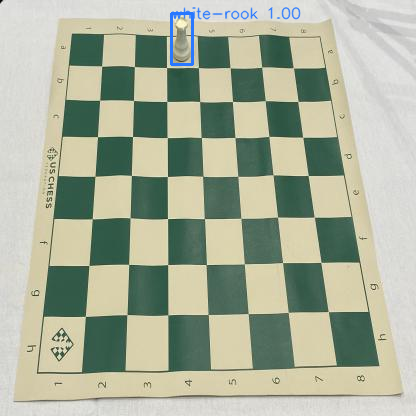
\includegraphics[width=\textwidth]{figures/faster_rcnn_prediction_4.png}
        \small Faster R-CNN
    \end{minipage}
    \caption{So sánh prediction trên test case 4.}
\end{figure}

Case 5 là một ảnh mà quân cờ nổi bật hơn. Cả ba mô hình đều bắt được object chính, nhưng YOLO và Faster R-CNN cho prediction rõ ràng và dễ đọc hơn. DETR vẫn phát hiện đúng quân chính nhưng nhìn chung ít box hơn và ít nhiễu hơn.

\begin{figure}[H]
    \centering
    \begin{minipage}[t]{0.32\textwidth}
        \centering
        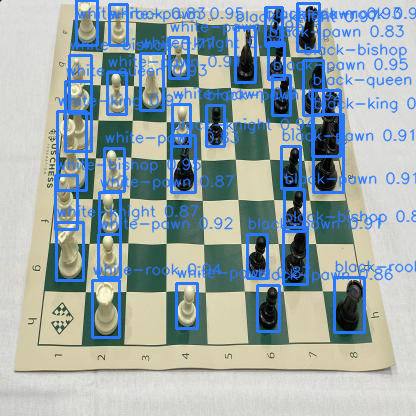
\includegraphics[width=\textwidth]{figures/yolo_prediction_5.png}
        \small YOLO
    \end{minipage}\hfill
    \begin{minipage}[t]{0.32\textwidth}
        \centering
        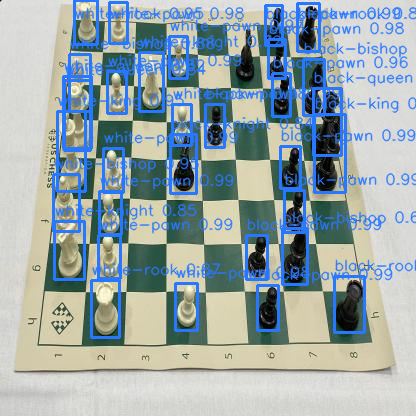
\includegraphics[width=\textwidth]{figures/detr_prediction_5.png}
        \small DETR
    \end{minipage}\hfill
    \begin{minipage}[t]{0.32\textwidth}
        \centering
        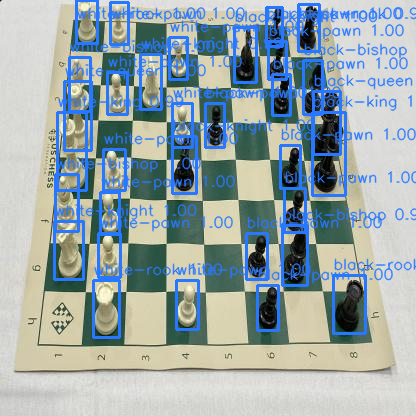
\includegraphics[width=\textwidth]{figures/faster_rcnn_prediction_5.png}
        \small Faster R-CNN
    \end{minipage}
    \caption{So sánh prediction trên test case 5.}
\end{figure}

\subsubsection{Đường cong đánh giá}

Ba đường cong dưới đây được tính trên cùng tập test và cùng dải confidence threshold, nên có thể dùng để so sánh trực tiếp. YOLO thường cho vùng cân bằng tốt hơn giữa precision và recall. Faster R-CNN có đường cong khá ổn định. DETR nhạy hơn với ngưỡng confidence và thiên về dự đoán ít box hơn, nên recall thường thấp hơn hai mô hình còn lại trong cấu hình hiện tại.

\begin{figure}[H]
    \centering
    \begin{minipage}[t]{0.32\textwidth}
        \centering
        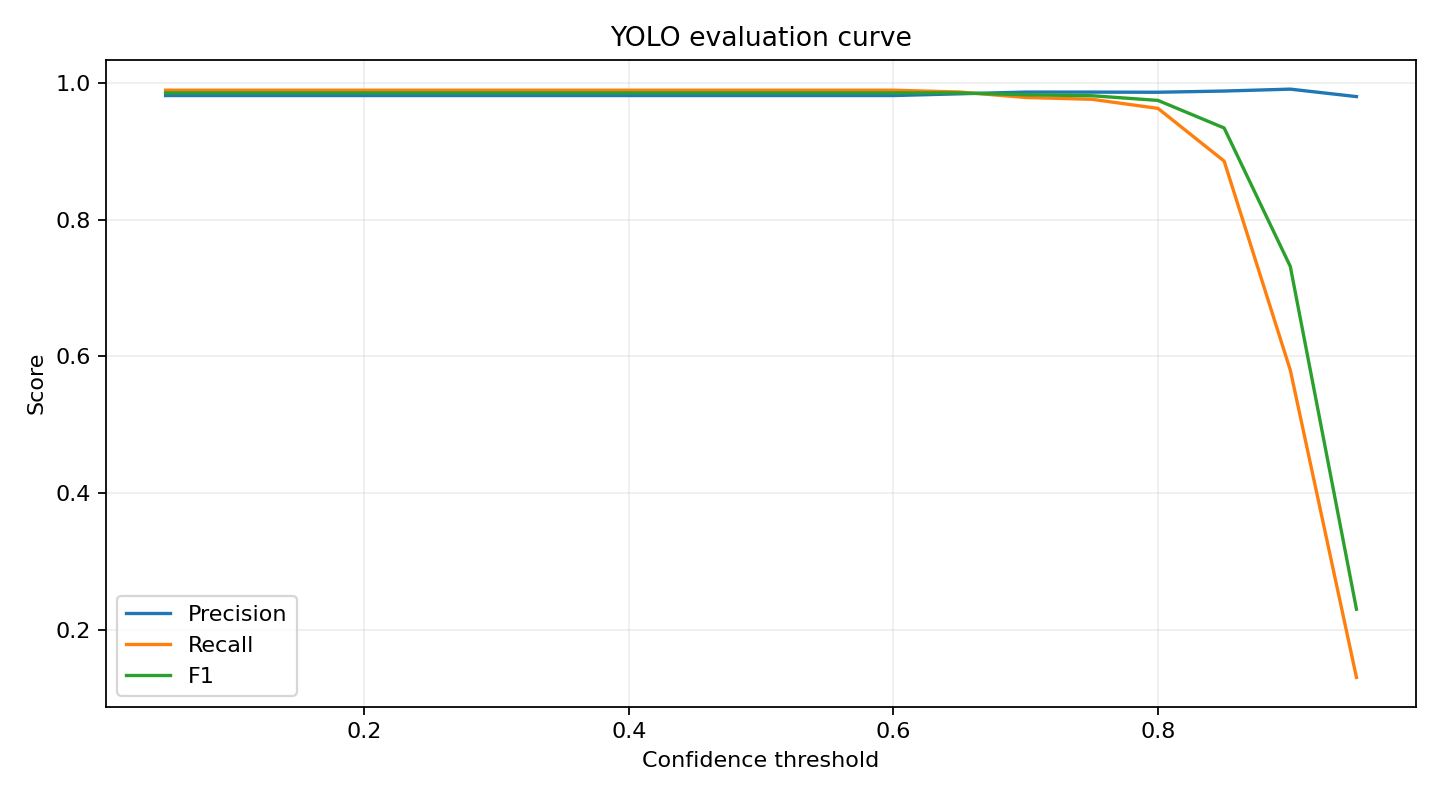
\includegraphics[width=\textwidth]{figures/yolo_eval_curve.png}
        \small YOLO
    \end{minipage}\hfill
    \begin{minipage}[t]{0.32\textwidth}
        \centering
        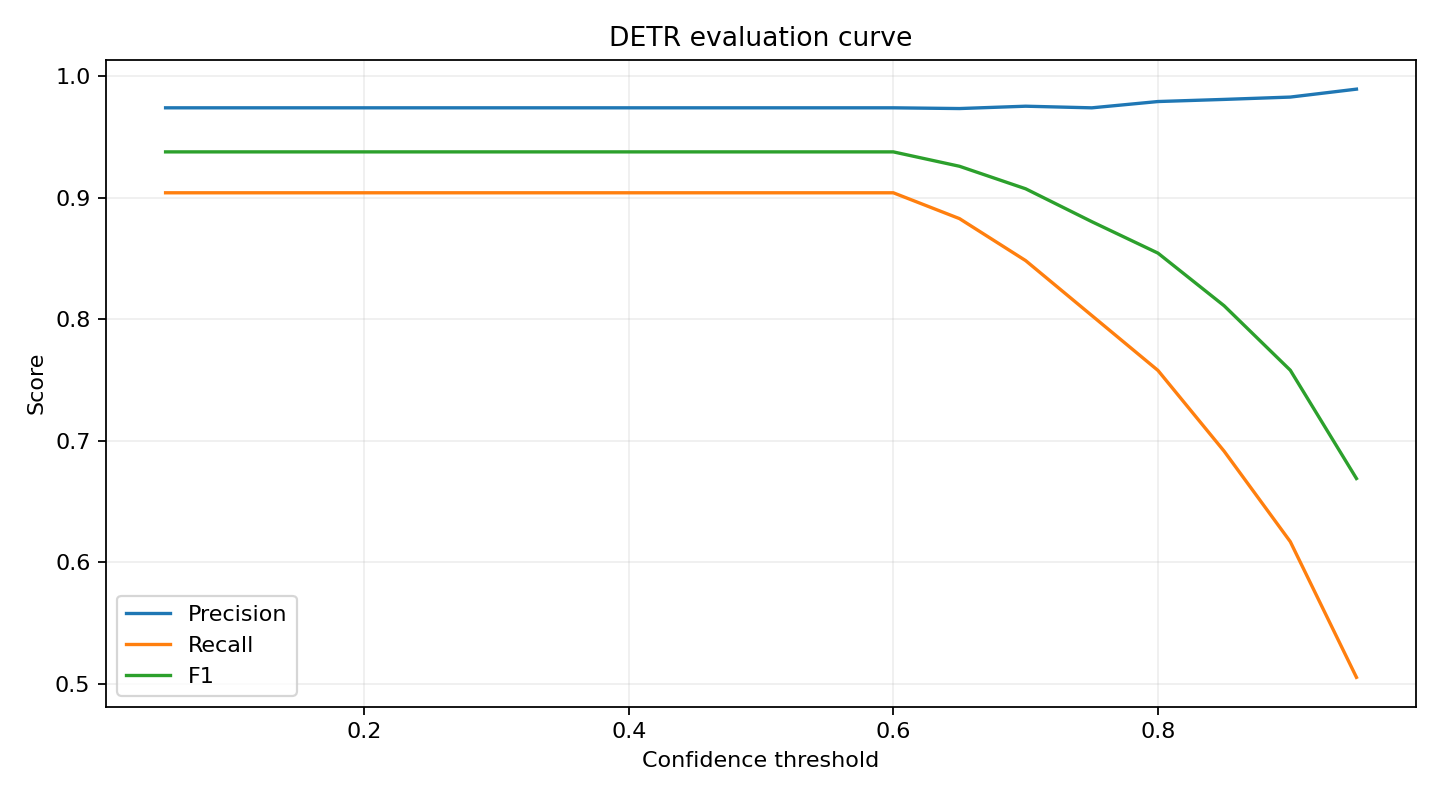
\includegraphics[width=\textwidth]{figures/detr_eval_curve.png}
        \small DETR
    \end{minipage}\hfill
    \begin{minipage}[t]{0.32\textwidth}
        \centering
        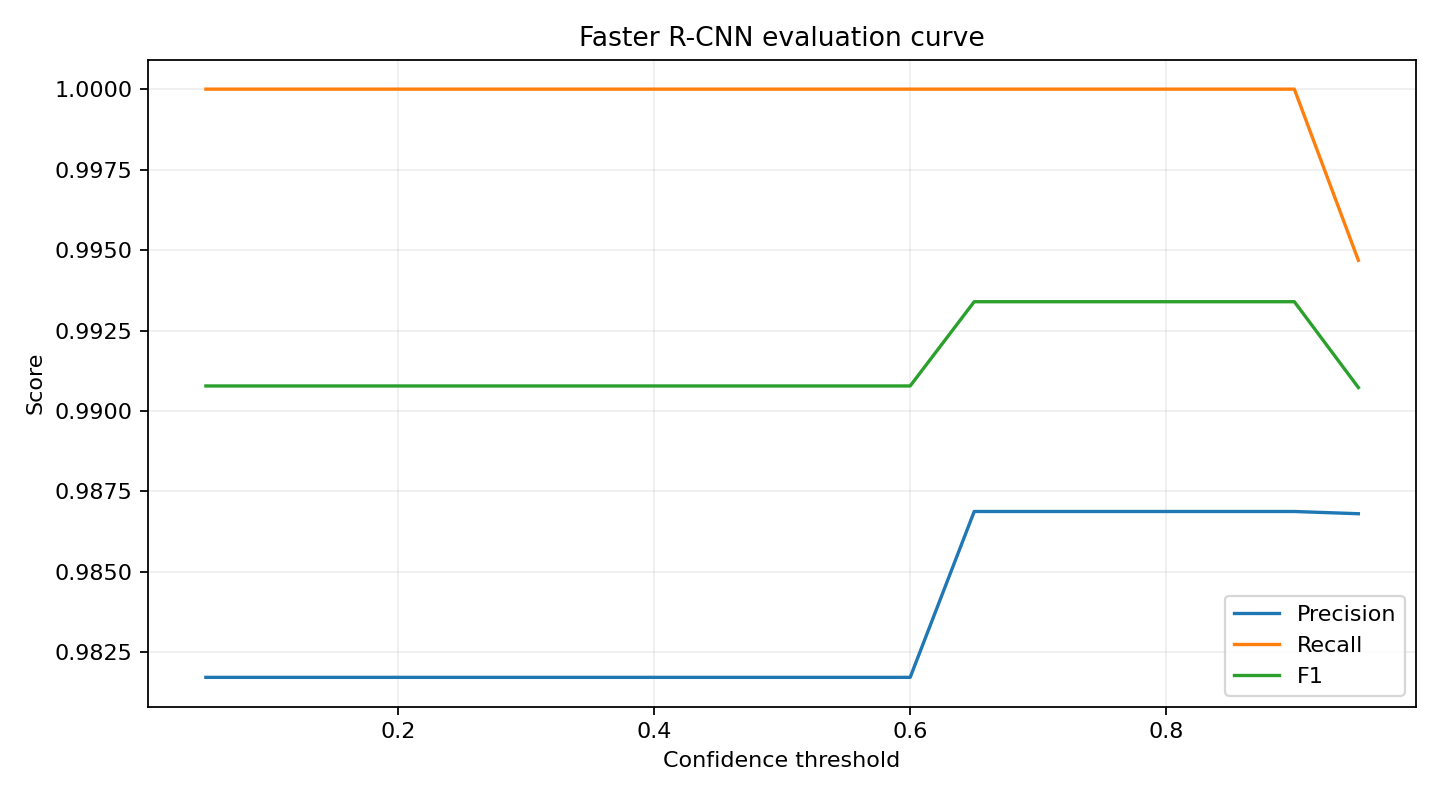
\includegraphics[width=\textwidth]{figures/faster_rcnn_eval_curve.png}
        \small Faster R-CNN
    \end{minipage}
    \caption{So sánh đường cong đánh giá của ba mô hình trên cùng tập test.}
\end{figure}

\subsubsection{Tổng hợp nhận xét}

Từ toàn bộ các hình so sánh, có thể rút ra ba điểm chính:
\begin{itemize}[leftmargin=1.2cm]
    \item YOLO là mô hình cân bằng nhất giữa tốc độ, độ phủ detection và tính dễ đọc của kết quả.
    \item DETR cho kết quả sạch nhưng thận trọng hơn, đặc biệt trên ảnh ít object hoặc object nhỏ, nên dễ có cảm giác "dự đoán ít".
    \item Faster R-CNN là baseline ổn định, thể hiện tốt trên các ảnh có nhiều quân cờ và giữ box khá đều.
\end{itemize}

Vì bài toán có phân bố lớp lệch, các lớp hiếm vẫn là điểm yếu chung của cả ba mô hình. Do đó, nhận xét chính của báo cáo không chỉ nằm ở số lượng box đúng, mà còn ở độ ổn định và khả năng giữ object trong các tình huống khó.

\subsection{Bảng tổng hợp nhận xét}

\begin{longtable}{p{0.18\textwidth}p{0.18\textwidth}p{0.54\textwidth}}
\toprule
\textbf{Mô hình} & \textbf{Đặc điểm nổi bật} & \textbf{Nhận xét} \\
\midrule
YOLO & One-stage, nhanh, trực quan & Phù hợp nhất cho bài toán cần tốc độ và ảnh prediction dễ đọc. Kết quả khá ổn trên quân cờ phổ biến. \\
DETR & Transformer, set prediction & Hiện đại và sạch về mặt pipeline, nhưng nhạy với cấu hình train và dữ liệu nhỏ. Cần cấu hình cẩn thận để ổn định. \\
Faster R-CNN & Two-stage, ổn định & Cho kết quả cân bằng, dễ kiểm soát, phù hợp làm baseline mạnh trong báo cáo học thuật. \\
\bottomrule
\end{longtable}

Nhìn chung, YOLO là mô hình có tính thực dụng cao nhất trong bài này. Faster R-CNN cho chất lượng ổn định, còn DETR thể hiện đúng tinh thần của một mô hình transformer hiện đại nhưng đòi hỏi điều chỉnh hyperparameter cẩn thận hơn. Trên bộ dữ liệu có phân bố lớp lệch như bài toán cờ vua, các lớp hiếm vẫn là điểm khó chung của cả ba mô hình.

\section{Kết luận}

Bài thực hành 03 đã hoàn thành việc xây dựng pipeline phát hiện đối tượng trên bộ dữ liệu Chess Pieces với ba mô hình YOLO, DETR và Faster R-CNN. Nhóm đã chuẩn hóa dữ liệu sang các định dạng cần thiết, huấn luyện các mô hình, xuất hình prediction và tổng hợp kết quả để so sánh trực quan.

Qua thực nghiệm, nhóm quan sát được ba điểm chính. Thứ nhất, bộ dữ liệu có tính mất cân bằng rõ rệt nên các lớp hiếm khó được mô hình học tốt như các lớp xuất hiện nhiều. Thứ hai, YOLO cho tốc độ và tính ổn định cao, phù hợp với mục tiêu triển khai nhanh. Thứ ba, DETR và Faster R-CNN đều mang lại góc nhìn thú vị về detection hiện đại, trong đó DETR cho thấy đặc trưng end-to-end còn Faster R-CNN thể hiện sự ổn định của detector hai giai đoạn.

Về mặt học thuật, bài thực hành giúp nhóm hiểu rõ hơn sự khác nhau giữa các họ mô hình phát hiện đối tượng, vai trò của định dạng annotation và ảnh hưởng của ngưỡng confidence khi trực quan hóa kết quả. Trong ứng dụng thực tế, việc chọn mô hình sẽ phụ thuộc vào yêu cầu về tốc độ, độ ổn định và mức độ phù hợp với dữ liệu đầu vào.

\end{document}
